\documentclass[11pt]{article}
\usepackage[letterpaper,margin=1in]{geometry}
\usepackage[sc]{mathpazo}
\usepackage{amsmath,amssymb,booktabs,graphicx,caption}
\usepackage[hidelinks,pdfstartview=FitH]{hyperref}
\newcommand{\trainmin}{28}
\newcommand{\nsteps}{24,000}
\newcommand{\nouter}{600}
\newcommand{\ninner}{40}
\newcommand{\evalpaper}{0.16}
\newcommand{\evaldense}{0.48}
\newcommand{\resV}{7.8e-4}
\newcommand{\resq}{1.3e-3}
\newcommand{\resVmax}{1.1e-2}
\newcommand{\resqmax}{2.0e-2}

\title{A Physics-Informed Neural Network Solution of the\\ Diffusion Model of Partial Default}
\author{Grok Bot}
\date{November 2026}
\begin{document}
\maketitle

\noindent This note solves the main calibration of the quantitative diffusion model of partial default (Kim and
Mihalache) with a physics-informed neural network (PINN) in PyTorch, from scratch, and compares the solution with the
converged implicit upwind finite-difference (FD) solution of the C++/CUDA port of the replication package. The code is in
the repository \texttt{Partial-Default-PINN}.

\section{The equations}

The state is debt $B\in[0,1]$ and log endowment $z\in[\underline z,\overline z]$, $\overline z=-\underline z=2.5$
stationary standard deviations, with $dz=-\mu z\,dt+\sigma dW$ reflected at both ends. The value $V(B,z)$ and the bond
price $q(B,z)$ solve the stationary HJB and pricing equations
\begin{align*}
\rho V &= \max_{d\in[0,1],\,S\in\mathcal S(d,q,B,z)} \Big\{u(c)+S\,V_B\Big\} - \mu z V_z + \tfrac{\sigma^2}{2} V_{zz},\\
\xi(d)\,q &= (1-d)(\delta+\lambda) + S\,q_B - \mu z\,q_z + \tfrac{\sigma^2}{2} q_{zz},
\qquad \xi(d) = r+\delta-\kappa(\delta+\lambda)d,
\end{align*}
with $c = \phi(d,z)e^z-(1-d)(\delta+\lambda)B + q\,\big(S+(\delta-\kappa(\delta+\lambda)d)B\big)$, $u(c)=-1/c$, and the
admissible set $\mathcal S$ given by the consumption floor, $|S|\le 1$, the underwriting standard (new issuance capped by
$L(q)$, zero below $\underline q$, rising over the band), and the state constraints $S\ge 0$ at $B=0$ and $S\le 0$ at
$B=1$. The reflecting barriers give $V_z=q_z=0$ at $\underline z,\overline z$. All parameters are those of
\texttt{data/ou\_main.npz} of the replication package.

\section{Method}

\paragraph{Networks.} $V$ and $q$ are two fully connected networks (4 hidden layers of 128 $\tanh$ units each),
$V=-20+2N_V$ and $q=\mathrm{sigmoid}(N_q)$. The inputs are $2B-1$, $2B^{3/2}-1$, and $\cos(k\pi s)$, $k=1,\dots,8$,
with $s=(z-\underline z)/(\overline z-\underline z)$. Every function of the cosine features has a zero derivative in
$z$ at both barriers, so the Neumann conditions hold exactly for any weights, and the eight frequencies resolve the
boundary layers that the reflection creates next to the barriers. The $B^{3/2}$ input lets $V_B$ move like
$\sqrt B$ next to the state constraint at $B=0$, where a saving borrower's drift vanishes like $-\sqrt B$. There are no
boundary conditions in $B$: the drift points into the domain at both ends.

\paragraph{The node problem.} Given $(V_B,q)$ at a point, the policy $(S,c,d)$ maximizes the Hamiltonian exactly as in
the replication package (\texttt{pdmodel.best\_node}): the first-order condition for $c$ clamped to the admissible
interval of $S$, the closed-form interior default intensity where it is admissible, and otherwise a golden-section
search over $d$ with the candidates $d=0$ and $d=1$. The PINN uses the exact derivative $V_B$ of the network in place of
the one-sided differences of the upwind scheme. The routine is vectorized over points in PyTorch, evaluated in double
precision, and agrees with the package's routine to $10^{-15}$ on random inputs (\texttt{tests/test\_node.py}).

\paragraph{Pseudo-time stepping.} The solution is the stationary point of the implicit scheme of the paper, with the
linear solves replaced by least-squares fits of the networks. At outer step $k$ (pseudo-time step $\Delta t_k$), frozen
copies $(V^k,q^k)$ give the policy at every collocation point, and the networks are trained for \ninner{} Adam steps,
on fresh collocation points each step, to minimize the residuals of
\begin{align*}
(\rho+\tfrac1{\Delta t})V - S^kV_B + \mu zV_z - \tfrac{\sigma^2}{2}V_{zz} &= u(c^k) + \tfrac1{\Delta t}V^k,\\
(\xi(d^k)+\tfrac1{\Delta t})q - S^kq_B + \mu z q_z - \tfrac{\sigma^2}{2}q_{zz} &= (1-d^k)(\delta+\lambda) + \tfrac1{\Delta t}q^k,
\end{align*}
each divided by its diagonal coefficient so that both are in the units of the unknown. Given the policy the two
problems are linear and separate, so there is no weighting of $V$ against $q$ to choose. The frozen copies are taken
from an exponential moving average of the weights (decay 0.99 per Adam step), which damps the noise of the stochastic
fits before it reaches the policy. $\Delta t$ starts at 0.05 and grows by 3\% per outer step to 1; the learning rate is
$10^{-3}$ until $\Delta t$ reaches its cap and then decays geometrically to $10^{-5}$. The run has \nouter{} outer
steps (\nsteps{} Adam steps), starting from the package's initial guess (consuming $y-\lambda B$ forever, and the
static price), fitted to the networks first. The FD solution is not used in training.

\paragraph{The derivative of the HJB residual.} Where the drift vanishes, at the zero-drift locus on which the ergodic
mass concentrates, the HJB residual does not involve $V_B$, so it does not pin the policy. Its derivative in $B$ does:
at $S=0$ it reads $(\rho+\frac1{\Delta t}-S_B)V_B=\dots$. The loss of the HJB therefore adds the squared derivative of
its residual in $B$ (central differences with step 0.002, scaled by the length 0.05), at points whose two neighbors lie
on the same side of the default threshold. The term vanishes at the solution; it changes no equation. The pricing
equation needs no such term, since at $S=0$ it pins $q$ itself.

\paragraph{Collocation points.} Each Adam step draws 4,096 points (with their two neighbors in $B$): 32\% uniform on
the domain; 30\% from the ergodic density of the current policy (computed every five outer steps on the paper grid with
the package's upwind generator, cells drawn by mass, uniform within the cell); 14\% in the cells where the current
default intensity jumps; 10\% on the barriers in $z$ and in the boundary layers next to them; 8\% in the layer
$B<0.05$; 4\% on $B=0$; and 2\% on $B=1$. Training runs in single precision on an NVIDIA T1000.

\paragraph{Evaluation.} The trained networks are evaluated at the nodes of the paper grid ($201\times75$) and of the
dense grid ($2000\times121$). The ergodic density is that of the package's upwind generator in the PINN drift, and
the moments are computed by the package's \texttt{pdmoments.combined\_moments} (exact ergodic moments, and 16
simulated paths of 25,000 years), for the PINN and, with the same code, for the FD solution of the same grid.

\section{Results}

Training takes \trainmin{} minutes. Evaluating the networks and the policy on the paper grid takes \evalpaper{} s, on
the dense grid \evaldense{} s. On the paper grid the residuals of the stationary equations, with the exact derivatives of
the networks and weighted by the ergodic density (root mean square), are \resV{} (HJB) and \resq{} (pricing); their
maxima are \resVmax{} and \resqmax.

\begin{table}[h]\centering\small
\caption{Moments of Table 2 of the paper: FD and PINN on the paper grid and on the dense grid. $^*$untargeted.}
\label{tab:moments}
\begin{tabular}{lcccc}
\toprule
 & \multicolumn{2}{c}{paper grid, $201\times 75$} & \multicolumn{2}{c}{dense grid, $2000\times 121$} \\
\cmidrule(lr){2-3}\cmidrule(lr){4-5}
moment & FD & PINN & FD & PINN \\
\midrule
frequency of partial default & 0.389 & 0.401 & 0.384 & 0.395 \\
mean partial default, in default & 0.477 & 0.465 & 0.480 & 0.472 \\
s.d. partial default, in default & 0.262 & 0.256 & 0.256 & 0.251 \\
mean debt / output & 0.300 & 0.304 & 0.299 & 0.303 \\
s.d. debt / output & 0.204 & 0.200 & 0.201 & 0.199 \\
mean debt service / output & 0.033 & 0.033 & 0.033 & 0.033 \\
s.d. debt service / output & 0.018 & 0.019 & 0.018 & 0.019 \\
mean debt due / output & 0.050 & 0.051 & 0.050 & 0.051 \\
s.d. spread & 0.029 & 0.028 & 0.029 & 0.028 \\
persistence of output & 0.929 & 0.929 & 0.929 & 0.929 \\
s.d. output & 0.105 & 0.105 & 0.105 & 0.105 \\
mean defaulted coupons / output$^*$ & 0.045 & 0.043 & 0.045 & 0.044 \\
s.d. defaulted coupons / output$^*$ & 0.034 & 0.032 & 0.033 & 0.032 \\
mean spread$^*$ & 0.020 & 0.019 & 0.019 & 0.019 \\
corr(spread, output)$^*$ & -0.757 & -0.760 & -0.758 & -0.761 \\
corr(spread, debt)$^*$ & 0.843 & 0.826 & 0.841 & 0.826 \\
s.d. consumption / s.d. output$^*$ & 0.926 & 0.927 & 0.927 & 0.927 \\
\midrule
loss & 0.2595 & 0.2516 & 0.2602 & 0.2541 \\
mass at $B=0$ & 0.058 & 0.080 & 0.044 & 0.073 \\
mean debt $E[B]$ & 0.284 & 0.288 & 0.284 & 0.288 \\
\bottomrule
\end{tabular}

\end{table}

\begin{table}[h]\centering\small
\caption{Absolute differences between the PINN and the FD solution at the grid nodes: maximum over the grid,
99th percentile over the nodes with ergodic mass, and mean weighted by the FD ergodic density.}
\label{tab:errors}
\begin{tabular}{lcccccc}
\toprule
 & \multicolumn{3}{c}{paper grid, $201\times 75$} & \multicolumn{3}{c}{dense grid, $2000\times 121$} \\
\cmidrule(lr){2-4}\cmidrule(lr){5-7}
object & max & 99th pct. & ergodic mean & max & 99th pct. & ergodic mean \\
\midrule
value $V$ & 1.2e-2 & 8.4e-3 & 3.1e-3 & 8.2e-3 & 5.5e-3 & 2.0e-3 \\
price $q$ & 2.8e-2 & 2.3e-2 & 3.8e-3 & 2.7e-2 & 2.1e-2 & 3.7e-3 \\
consumption $c$ & 3.5e-2 & 1.3e-2 & 2.0e-3 & 5.1e-2 & 1.4e-2 & 2.1e-3 \\
default intensity $d$ & 6.8e-1 & 1.6e-2 & 2.3e-3 & 6.8e-1 & 1.7e-2 & 2.2e-3 \\
drift $S$ & 4.0e-2 & 1.7e-2 & 2.4e-3 & 5.1e-2 & 1.8e-2 & 2.4e-3 \\
\midrule
ergodic density, $\sum|g-g^{FD}|$ & \multicolumn{3}{c}{0.190} & \multicolumn{3}{c}{0.205} \\
\bottomrule
\end{tabular}

\end{table}

Table~\ref{tab:moments} compares the moments and Table~\ref{tab:errors} the objects. Output moments, debt service,
debt due, the consumption ratio and the correlation of spreads with output agree with FD to two or three decimals.
The PINN's ergodic distribution carries slightly more debt (mean $B$ 0.288 against 0.284, debt/output 0.304 against
0.300; mass at $B=0$ 0.080 against 0.058), with spreads a little lower (mean 1.92\% against 1.98\%, s.d.\ 2.81\% against 2.95\%), partial default
somewhat more frequent (0.401 against 0.390) and shallower (0.465 against 0.477), and corr(spread, debt) 0.826
against 0.843. These differences trace to the price schedule just past the default threshold, where the PINN's $q$
is up to 0.03 above the FD price (Figure~\ref{fig:diff}). The same pattern holds on the dense grid. The largest pointwise
differences in $d$ sit on the default threshold, where the intensity jumps from zero to about 0.4: a node next to the
threshold can fall on either side. Figures~\ref{fig:overlay}--\ref{fig:contours} show the solutions.

\begin{figure}[p]\centering
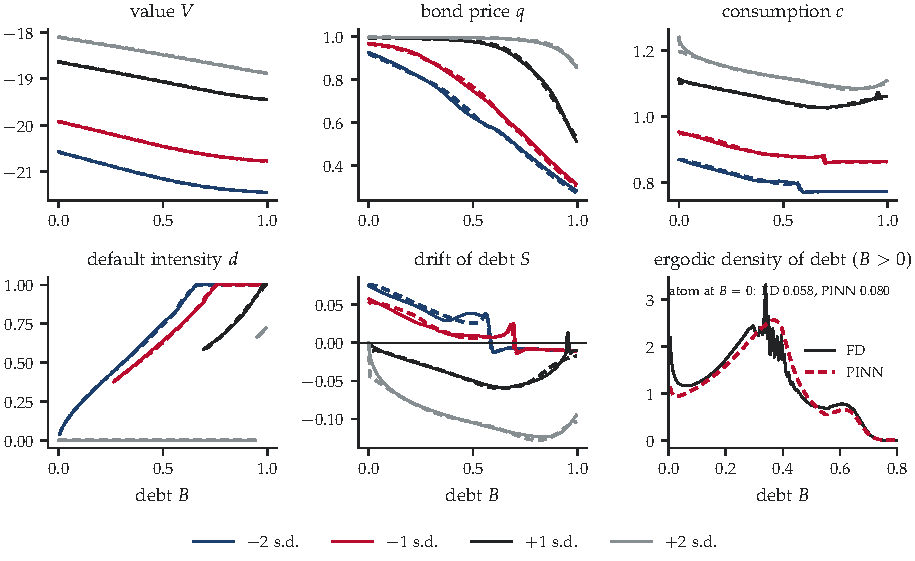
\includegraphics[width=\textwidth]{figures/overlay_paper.pdf}
\caption{FD (solid) and PINN (dashed) against debt at the four endowment levels of the paper's Figure~6, paper grid.
Last panel: the ergodic density of debt.}\label{fig:overlay}
\vspace{1em}
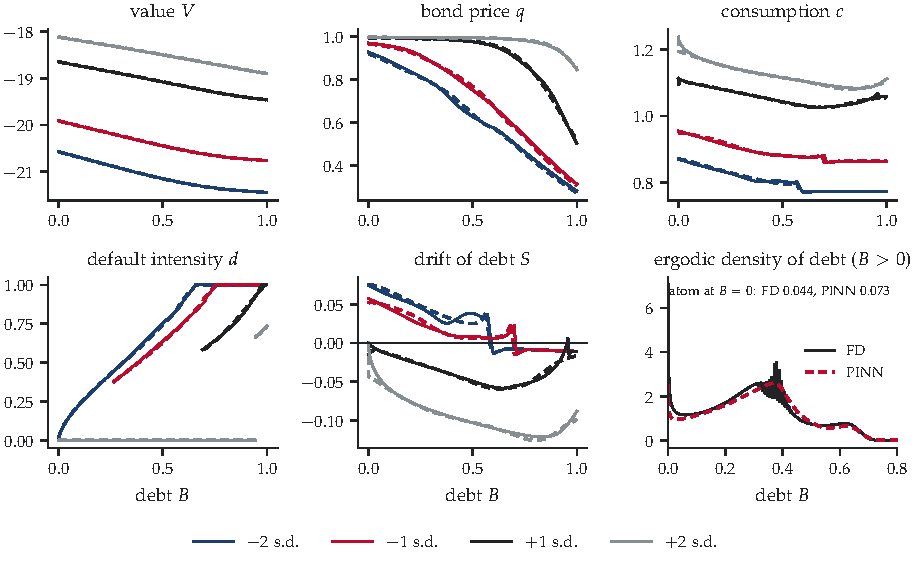
\includegraphics[width=\textwidth]{figures/overlay_dense.pdf}
\caption{As Figure~\ref{fig:overlay}, dense grid ($2000\times121$).}\label{fig:overlay_dense}
\end{figure}

\begin{figure}[p]\centering
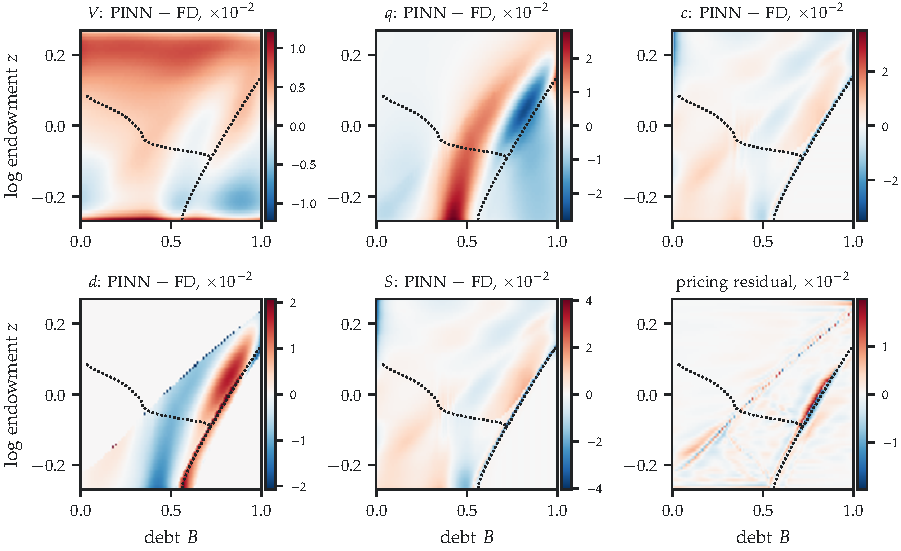
\includegraphics[width=\textwidth]{figures/diff_paper.pdf}
\caption{PINN minus FD in the $(B,z)$ plane, paper grid, and the PINN's pricing residual. Dotted: the FD zero-drift
locus.}\label{fig:diff}
\vspace{1em}
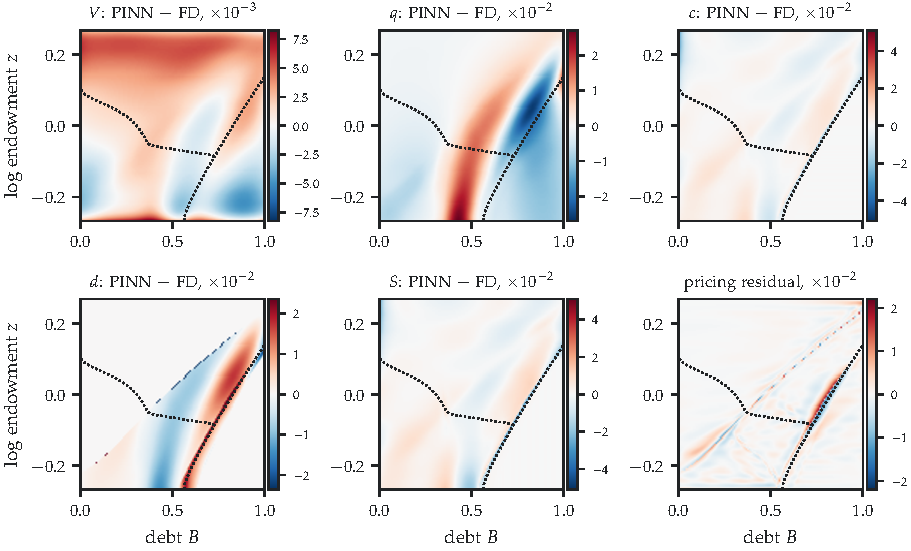
\includegraphics[width=\textwidth]{figures/diff_dense.pdf}
\caption{As Figure~\ref{fig:diff}, dense grid.}\label{fig:diff_dense}
\end{figure}

\begin{figure}[p]\centering
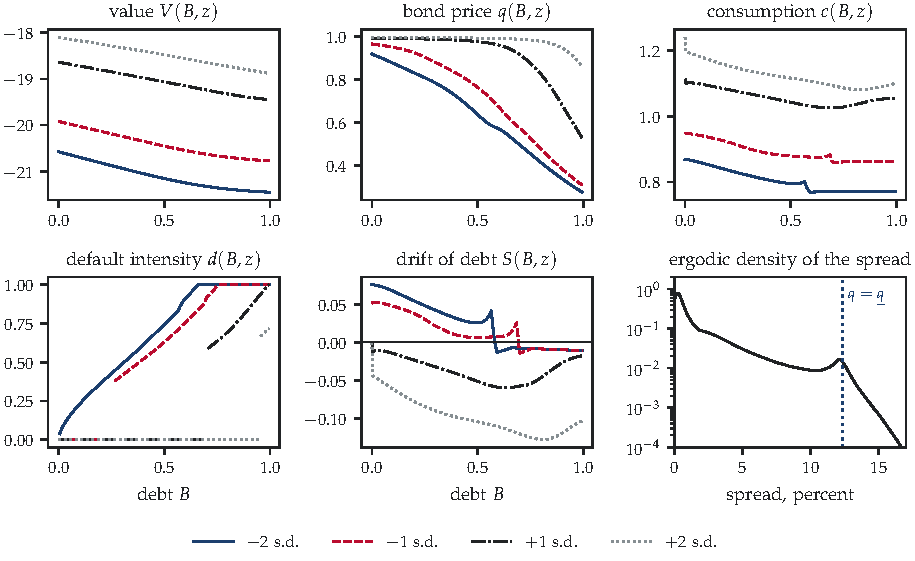
\includegraphics[width=\textwidth]{figures/ou_slices_pinn.pdf}
\caption{The paper's Figure 6 drawn by the package's code from the PINN solution (paper grid).}\label{fig:slices_pinn}
\vspace{1em}
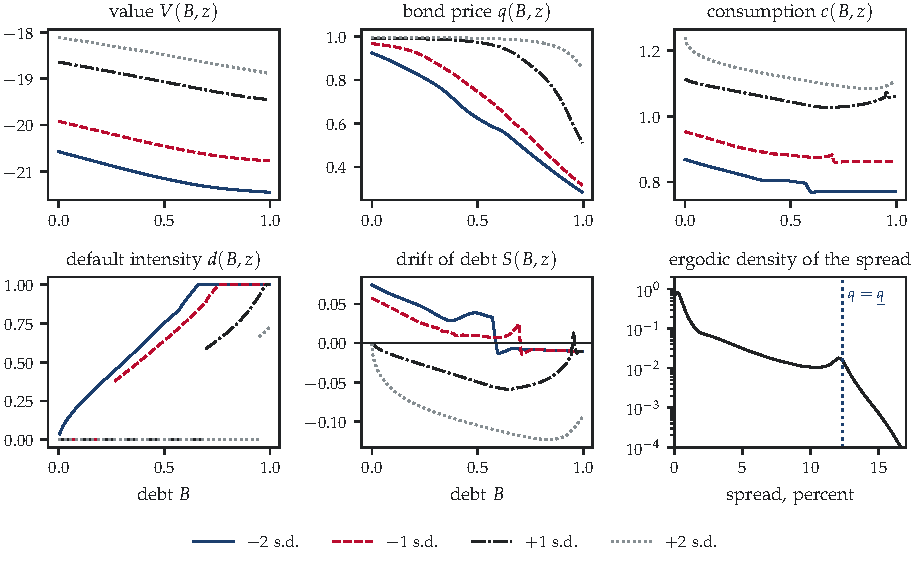
\includegraphics[width=\textwidth]{figures/ou_slices_fd.pdf}
\caption{The paper's Figure 6 from the FD solution (paper grid).}\label{fig:slices_fd}
\end{figure}

\begin{figure}[p]\centering
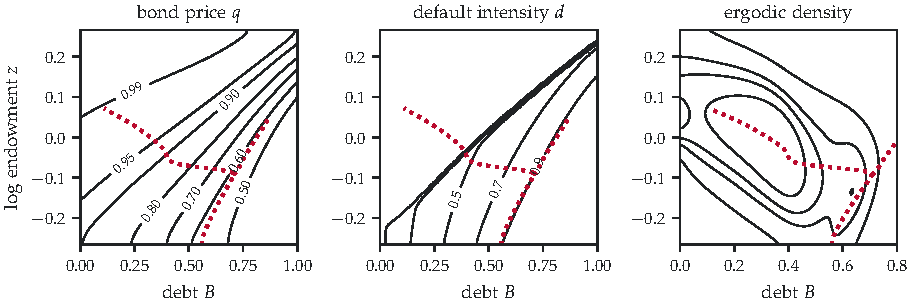
\includegraphics[width=\textwidth]{figures/ou_contours_pinn.pdf}
\caption{The paper's Figure 7 drawn by the package's code from the PINN solution (paper grid).}
\vspace{1em}
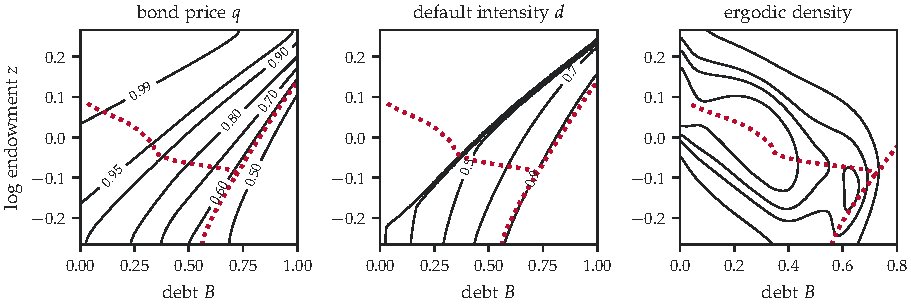
\includegraphics[width=\textwidth]{figures/ou_contours_fd.pdf}
\caption{The paper's Figure 7 from the FD solution (paper grid).}\label{fig:contours}
\vspace{1em}
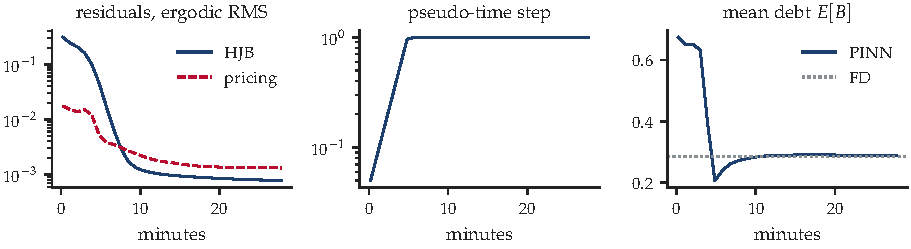
\includegraphics[width=\textwidth]{figures/training.pdf}
\caption{Training: ergodic RMS residuals, the pseudo-time step, and the mean debt of the PINN's ergodic density
(dotted: FD).}\label{fig:training}
\end{figure}

\end{document}
